% A fixture exercising most of what the converter has to handle.
\documentclass[aspectratio=43]{beamer}
\usetheme{Madrid}
\usepackage{amsmath, amssymb}
\usepackage{booktabs}
\usepackage{graphicx}
\usepackage{tikz}
\usepackage{pgfplots}
\pgfplotsset{compat=1.18}

\graphicspath{{figures/}{img/}}

\newcommand{\R}{\mathbb{R}}
\newcommand{\greet}[2][world]{Hello #1, meet #2}
\DeclareMathOperator{\argmin}{argmin}

\title{Beamer to PowerPoint}
\subtitle{A conversion fixture}
\author{A. Mohebbi}
\institute{Polytechnique Montr\'eal}
\date{\today}

\begin{document}

\begin{frame}
  \titlepage
\end{frame}

\section{Text and lists}

\begin{frame}{Bullets and inline styling}
  \begin{itemize}
    \item Plain item with \textbf{bold}, \emph{italic} and \texttt{monospace}
    \item An \alert{alerted} item and a \textcolor{blue}{blue} one
    \item Nested content
      \begin{itemize}
        \item Second level with inline math $E = mc^2$
        \item[$\star$] A custom marker
          \begin{itemize}
            \item Third level
          \end{itemize}
      \end{itemize}
    \item A link: \url{https://example.org} and \href{https://example.org}{named}
  \end{itemize}
\end{frame}

\begin{frame}{Overlays and blocks}
  \begin{block}{A standard block}
    Content revealed step by step.
  \end{block}
  \begin{itemize}
    \item First, always visible
    \pause
    \item Second, after one click
    \item<3-> Third, explicitly on step three
  \end{itemize}
  \begin{alertblock}{Careful}
    Macro expansion: \greet{you}. Operator: $\argmin_x f(x)$.
  \end{alertblock}
\end{frame}

\section{Mathematics}

\begin{frame}{Equations}
  Inline math such as $\sum_{i=1}^{n} x_i \in \R$ flows with the text.
  \[
    \frac{\partial u}{\partial t} = \alpha \nabla^2 u
  \]
  \begin{align}
    a &= b + c \\
    d &= e - f
  \end{align}
  A matrix:
  \[
    A = \begin{bmatrix} 1 & 2 \\ 3 & 4 \end{bmatrix}
  \]
\end{frame}

\section{Tables and figures}

\begin{frame}{A booktabs table}
  \begin{table}
    \centering
    \begin{tabular}{lrr}
      \toprule
      Method & Accuracy & Time (s) \\
      \midrule
      Baseline      & 0.812 & 12.4 \\
      \textbf{Ours} & 0.947 &  8.1 \\
      \midrule
      \multicolumn{2}{l}{Relative gain} & 34\% \\
      \bottomrule
    \end{tabular}
    \caption{Results on the held-out set.}
  \end{table}
\end{frame}

\begin{frame}{A raster figure}
  \begin{figure}
    \centering
    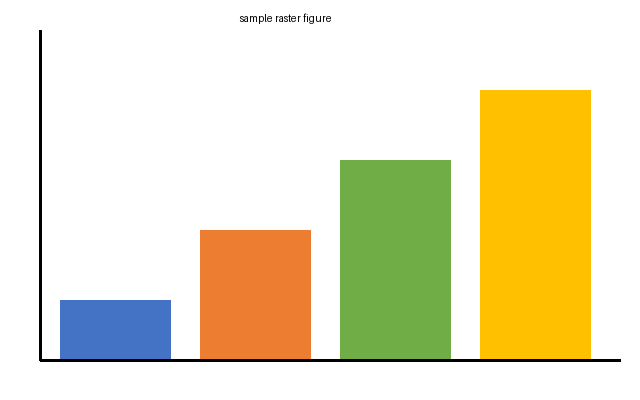
\includegraphics[width=0.6\textwidth]{sample.png}
    \caption{An included raster image.}
  \end{figure}
\end{frame}

\begin{frame}{TikZ and pgfplots}
  \begin{columns}
    \begin{column}{0.48\textwidth}
      \begin{tikzpicture}
        \draw[thick,->] (0,0) -- (2,0) node[right] {$x$};
        \draw[thick,->] (0,0) -- (0,2) node[above] {$y$};
        \filldraw[blue] (1,1) circle (2pt) node[above right] {$p$};
      \end{tikzpicture}
    \end{column}
    \begin{column}{0.48\textwidth}
      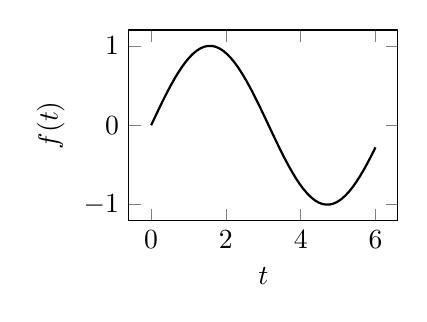
\begin{tikzpicture}
        \begin{axis}[width=5cm, height=4cm, xlabel=$t$, ylabel=$f(t)$]
          \addplot[domain=0:6, samples=60, thick] {sin(deg(x))};
        \end{axis}
      \end{tikzpicture}
    \end{column}
  \end{columns}
\end{frame}

% Pulled in with \input to exercise multi-file projects.
\begin{frame}{From an included file}
  \begin{columns}
    \begin{column}{0.5\textwidth}
      \begin{itemize}
        \item Left column
        \item Resolved through \texttt{graphicspath}
      \end{itemize}
    \end{column}
    \begin{column}{0.5\textwidth}
      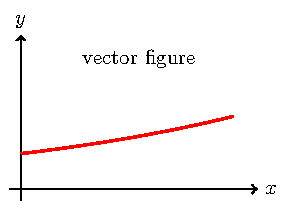
\includegraphics[width=\textwidth]{vector.pdf}
    \end{column}
  \end{columns}
\end{frame}

\begin{frame}{A theorem environment}
  \begin{theorem}[Convergence]
    The iteration converges whenever $\rho(A) < 1$.
  \end{theorem}
  \begin{description}
    \item[Input] a matrix $A \in \R^{n \times n}$
    \item[Output] the fixed point $x^\star$
  \end{description}
\end{frame}


\begin{frame}[fragile]{Verbatim}
  \begin{verbatim}
def convert(tex):
    return pptx  % not a comment
  \end{verbatim}
  Inline \verb|code $x$| stays literal.
\end{frame}

\end{document}
